% Options for packages loaded elsewhere
\PassOptionsToPackage{unicode}{hyperref}
\PassOptionsToPackage{hyphens}{url}
%
\documentclass[
]{article}
\usepackage{amsmath,amssymb}
\usepackage{lmodern}
\usepackage{iftex}
\ifPDFTeX
  \usepackage[T1]{fontenc}
  \usepackage[utf8]{inputenc}
  \usepackage{textcomp} % provide euro and other symbols
\else % if luatex or xetex
  \usepackage{unicode-math}
  \defaultfontfeatures{Scale=MatchLowercase}
  \defaultfontfeatures[\rmfamily]{Ligatures=TeX,Scale=1}
\fi
% Use upquote if available, for straight quotes in verbatim environments
\IfFileExists{upquote.sty}{\usepackage{upquote}}{}
\IfFileExists{microtype.sty}{% use microtype if available
  \usepackage[]{microtype}
  \UseMicrotypeSet[protrusion]{basicmath} % disable protrusion for tt fonts
}{}
\makeatletter
\@ifundefined{KOMAClassName}{% if non-KOMA class
  \IfFileExists{parskip.sty}{%
    \usepackage{parskip}
  }{% else
    \setlength{\parindent}{0pt}
    \setlength{\parskip}{6pt plus 2pt minus 1pt}}
}{% if KOMA class
  \KOMAoptions{parskip=half}}
\makeatother
\usepackage{xcolor}
\usepackage[margin=1in]{geometry}
\usepackage{color}
\usepackage{fancyvrb}
\newcommand{\VerbBar}{|}
\newcommand{\VERB}{\Verb[commandchars=\\\{\}]}
\DefineVerbatimEnvironment{Highlighting}{Verbatim}{commandchars=\\\{\}}
% Add ',fontsize=\small' for more characters per line
\usepackage{framed}
\definecolor{shadecolor}{RGB}{248,248,248}
\newenvironment{Shaded}{\begin{snugshade}}{\end{snugshade}}
\newcommand{\AlertTok}[1]{\textcolor[rgb]{0.94,0.16,0.16}{#1}}
\newcommand{\AnnotationTok}[1]{\textcolor[rgb]{0.56,0.35,0.01}{\textbf{\textit{#1}}}}
\newcommand{\AttributeTok}[1]{\textcolor[rgb]{0.77,0.63,0.00}{#1}}
\newcommand{\BaseNTok}[1]{\textcolor[rgb]{0.00,0.00,0.81}{#1}}
\newcommand{\BuiltInTok}[1]{#1}
\newcommand{\CharTok}[1]{\textcolor[rgb]{0.31,0.60,0.02}{#1}}
\newcommand{\CommentTok}[1]{\textcolor[rgb]{0.56,0.35,0.01}{\textit{#1}}}
\newcommand{\CommentVarTok}[1]{\textcolor[rgb]{0.56,0.35,0.01}{\textbf{\textit{#1}}}}
\newcommand{\ConstantTok}[1]{\textcolor[rgb]{0.00,0.00,0.00}{#1}}
\newcommand{\ControlFlowTok}[1]{\textcolor[rgb]{0.13,0.29,0.53}{\textbf{#1}}}
\newcommand{\DataTypeTok}[1]{\textcolor[rgb]{0.13,0.29,0.53}{#1}}
\newcommand{\DecValTok}[1]{\textcolor[rgb]{0.00,0.00,0.81}{#1}}
\newcommand{\DocumentationTok}[1]{\textcolor[rgb]{0.56,0.35,0.01}{\textbf{\textit{#1}}}}
\newcommand{\ErrorTok}[1]{\textcolor[rgb]{0.64,0.00,0.00}{\textbf{#1}}}
\newcommand{\ExtensionTok}[1]{#1}
\newcommand{\FloatTok}[1]{\textcolor[rgb]{0.00,0.00,0.81}{#1}}
\newcommand{\FunctionTok}[1]{\textcolor[rgb]{0.00,0.00,0.00}{#1}}
\newcommand{\ImportTok}[1]{#1}
\newcommand{\InformationTok}[1]{\textcolor[rgb]{0.56,0.35,0.01}{\textbf{\textit{#1}}}}
\newcommand{\KeywordTok}[1]{\textcolor[rgb]{0.13,0.29,0.53}{\textbf{#1}}}
\newcommand{\NormalTok}[1]{#1}
\newcommand{\OperatorTok}[1]{\textcolor[rgb]{0.81,0.36,0.00}{\textbf{#1}}}
\newcommand{\OtherTok}[1]{\textcolor[rgb]{0.56,0.35,0.01}{#1}}
\newcommand{\PreprocessorTok}[1]{\textcolor[rgb]{0.56,0.35,0.01}{\textit{#1}}}
\newcommand{\RegionMarkerTok}[1]{#1}
\newcommand{\SpecialCharTok}[1]{\textcolor[rgb]{0.00,0.00,0.00}{#1}}
\newcommand{\SpecialStringTok}[1]{\textcolor[rgb]{0.31,0.60,0.02}{#1}}
\newcommand{\StringTok}[1]{\textcolor[rgb]{0.31,0.60,0.02}{#1}}
\newcommand{\VariableTok}[1]{\textcolor[rgb]{0.00,0.00,0.00}{#1}}
\newcommand{\VerbatimStringTok}[1]{\textcolor[rgb]{0.31,0.60,0.02}{#1}}
\newcommand{\WarningTok}[1]{\textcolor[rgb]{0.56,0.35,0.01}{\textbf{\textit{#1}}}}
\usepackage{graphicx}
\makeatletter
\def\maxwidth{\ifdim\Gin@nat@width>\linewidth\linewidth\else\Gin@nat@width\fi}
\def\maxheight{\ifdim\Gin@nat@height>\textheight\textheight\else\Gin@nat@height\fi}
\makeatother
% Scale images if necessary, so that they will not overflow the page
% margins by default, and it is still possible to overwrite the defaults
% using explicit options in \includegraphics[width, height, ...]{}
\setkeys{Gin}{width=\maxwidth,height=\maxheight,keepaspectratio}
% Set default figure placement to htbp
\makeatletter
\def\fps@figure{htbp}
\makeatother
\setlength{\emergencystretch}{3em} % prevent overfull lines
\providecommand{\tightlist}{%
  \setlength{\itemsep}{0pt}\setlength{\parskip}{0pt}}
\setcounter{secnumdepth}{-\maxdimen} % remove section numbering
\ifLuaTeX
  \usepackage{selnolig}  % disable illegal ligatures
\fi
\IfFileExists{bookmark.sty}{\usepackage{bookmark}}{\usepackage{hyperref}}
\IfFileExists{xurl.sty}{\usepackage{xurl}}{} % add URL line breaks if available
\urlstyle{same} % disable monospaced font for URLs
\hypersetup{
  pdftitle={Advanced Macro 2 - Assignment 1},
  pdfauthor={Unterweger L., Oberbrinkmann S.},
  hidelinks,
  pdfcreator={LaTeX via pandoc}}

\title{Advanced Macro 2 - Assignment 1}
\author{Unterweger L., Oberbrinkmann S.}
\date{2023-03-30}

\begin{document}
\maketitle

\hypertarget{preliminary}{%
\section{Preliminary}\label{preliminary}}

We hereby declare that the answers to the given assignment are entirely
our own, resulting from our own work effort only. Our team members
contributed to the answers of the assignment in the following
proportions:\textbackslash{}

\begin{itemize}
  \item Unterweger Lucas: 50%
  \item Oberbrinkmann Sophia: 50%
\end{itemize}

\hypertarget{question-1-business-cycles-stylized-facts-4-points}{%
\section{Question 1: Business cycles stylized facts (4
Points)}\label{question-1-business-cycles-stylized-facts-4-points}}

We'll start by setting up our coding environment by importing necessary
packages. (Code not shown.)

Now, we can import and clean our data set.

\begin{Shaded}
\begin{Highlighting}[]
\NormalTok{ireland }\OtherTok{\textless{}{-}} \FunctionTok{read\_excel}\NormalTok{(}\StringTok{"data/Ireland\_GDPData.xlsx"}\NormalTok{, }\AttributeTok{sheet =} \DecValTok{4}\NormalTok{)}
\end{Highlighting}
\end{Shaded}

\begin{verbatim}
## New names:
## * `` -> `...1`
\end{verbatim}

\begin{Shaded}
\begin{Highlighting}[]
\FunctionTok{colnames}\NormalTok{(ireland) }\OtherTok{\textless{}{-}} \FunctionTok{c}\NormalTok{(}\StringTok{"t"}\NormalTok{,}\StringTok{"Y"}\NormalTok{,}\StringTok{"G"}\NormalTok{,}\StringTok{"C"}\NormalTok{,}\StringTok{"I"}\NormalTok{)}
\FunctionTok{head}\NormalTok{(ireland)}
\end{Highlighting}
\end{Shaded}

\begin{verbatim}
## # A tibble: 6 x 5
##   t            Y     G     C     I
##   <chr>    <dbl> <dbl> <dbl> <dbl>
## 1 1995-Q1 19924. 4407. 8996. 3573.
## 2 1995-Q2 20344. 4281. 9243. 3754.
## 3 1995-Q3 20559. 4288. 9470. 4123.
## 4 1995-Q4 20866  4138. 9628. 4168.
## 5 1996-Q1 21485. 4561. 9773  4158.
## 6 1996-Q2 21964. 4419. 9879. 4636.
\end{verbatim}

\begin{Shaded}
\begin{Highlighting}[]
\NormalTok{GDP }\OtherTok{\textless{}{-}} \FunctionTok{ts}\NormalTok{(ireland}\SpecialCharTok{$}\NormalTok{Y, }\AttributeTok{start =} \FloatTok{1995.0}\NormalTok{, }\AttributeTok{frequency =} \DecValTok{4}\NormalTok{)}
\NormalTok{C }\OtherTok{\textless{}{-}} \FunctionTok{ts}\NormalTok{(ireland}\SpecialCharTok{$}\NormalTok{C, }\AttributeTok{start =} \FloatTok{1995.0}\NormalTok{, }\AttributeTok{frequency =} \DecValTok{4}\NormalTok{)}
\NormalTok{I }\OtherTok{\textless{}{-}} \FunctionTok{ts}\NormalTok{(ireland}\SpecialCharTok{$}\NormalTok{I, }\AttributeTok{start =} \FloatTok{1995.0}\NormalTok{, }\AttributeTok{frequency =} \DecValTok{4}\NormalTok{)}
\NormalTok{G }\OtherTok{\textless{}{-}} \FunctionTok{ts}\NormalTok{(ireland}\SpecialCharTok{$}\NormalTok{G, }\AttributeTok{start =} \FloatTok{1995.0}\NormalTok{, }\AttributeTok{frequency =} \DecValTok{4}\NormalTok{)}
\FunctionTok{plot}\NormalTok{(GDP)}
\end{Highlighting}
\end{Shaded}

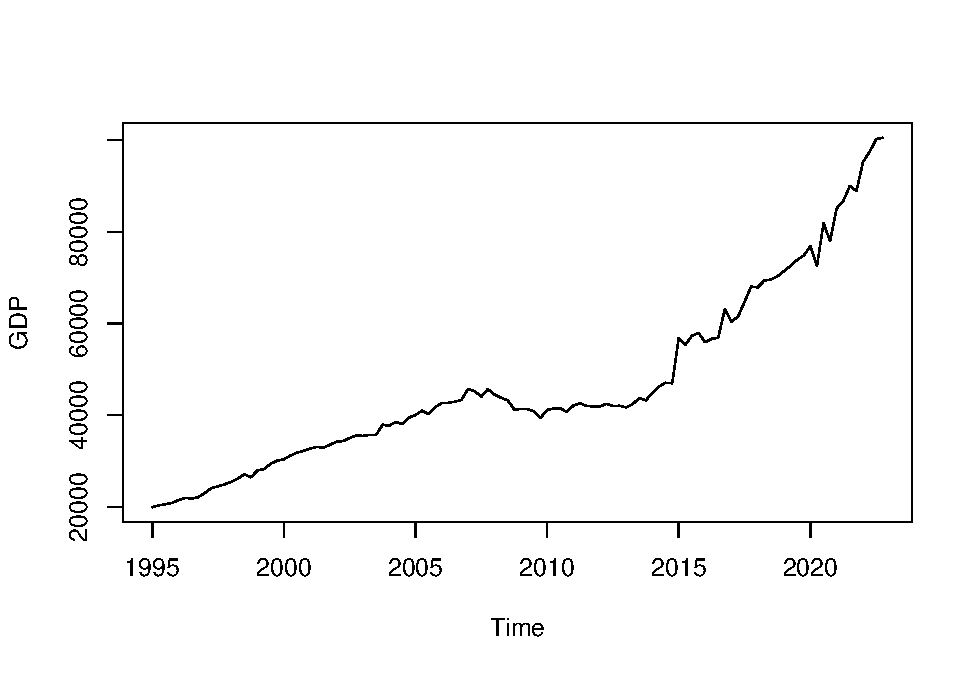
\includegraphics{AdvMacro2_Assignment1_files/figure-latex/unnamed-chunk-2-1.pdf}

\begin{Shaded}
\begin{Highlighting}[]
\FunctionTok{plot}\NormalTok{(C)}
\end{Highlighting}
\end{Shaded}

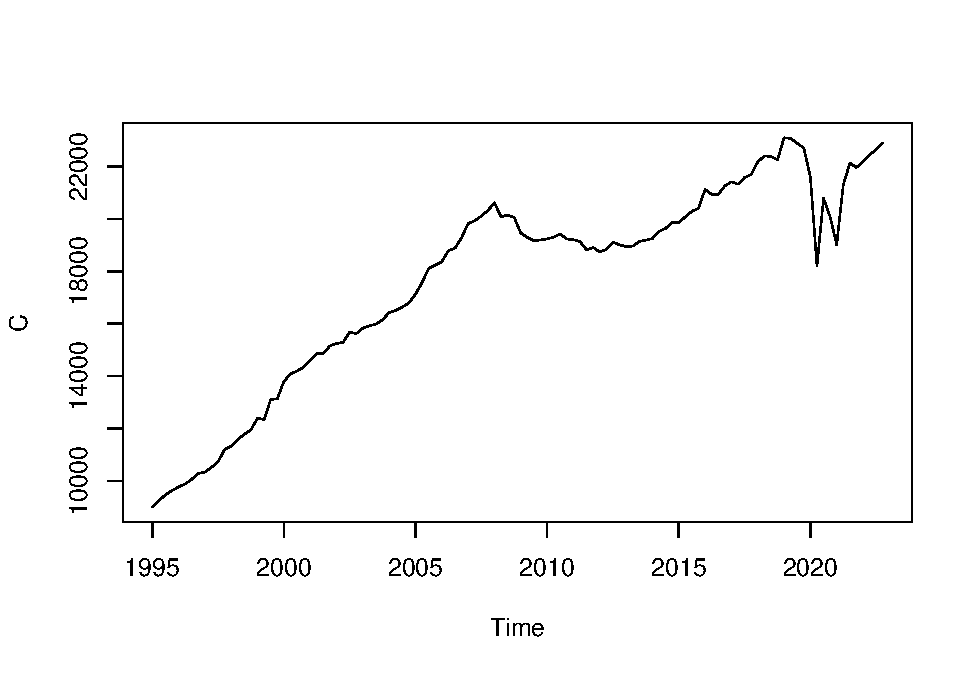
\includegraphics{AdvMacro2_Assignment1_files/figure-latex/unnamed-chunk-2-2.pdf}

\begin{Shaded}
\begin{Highlighting}[]
\FunctionTok{plot}\NormalTok{(I)}
\end{Highlighting}
\end{Shaded}

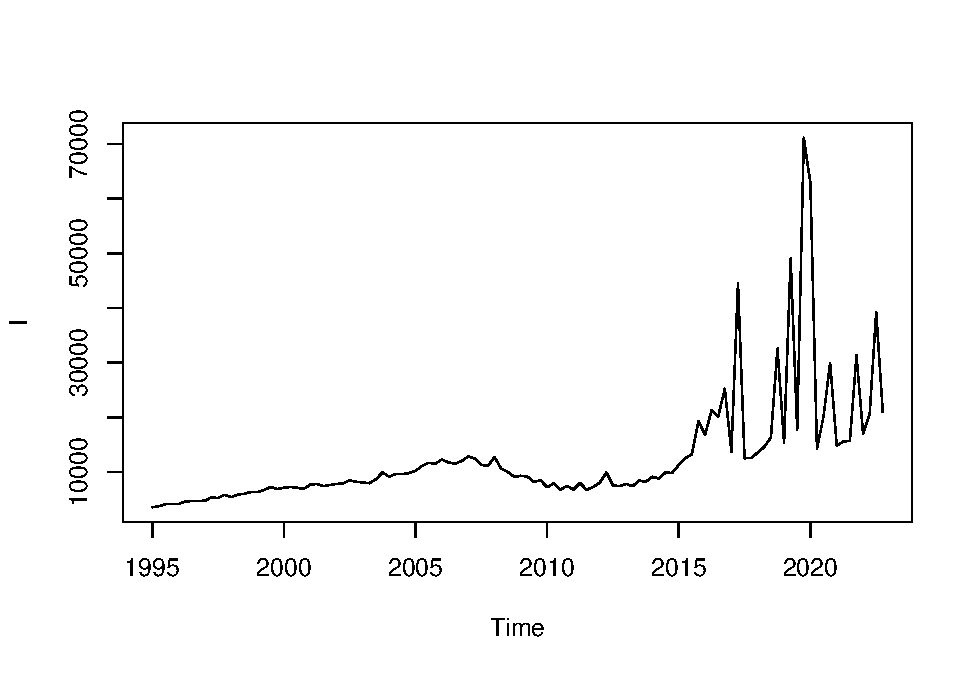
\includegraphics{AdvMacro2_Assignment1_files/figure-latex/unnamed-chunk-2-3.pdf}

\begin{Shaded}
\begin{Highlighting}[]
\FunctionTok{plot}\NormalTok{(G)}
\end{Highlighting}
\end{Shaded}

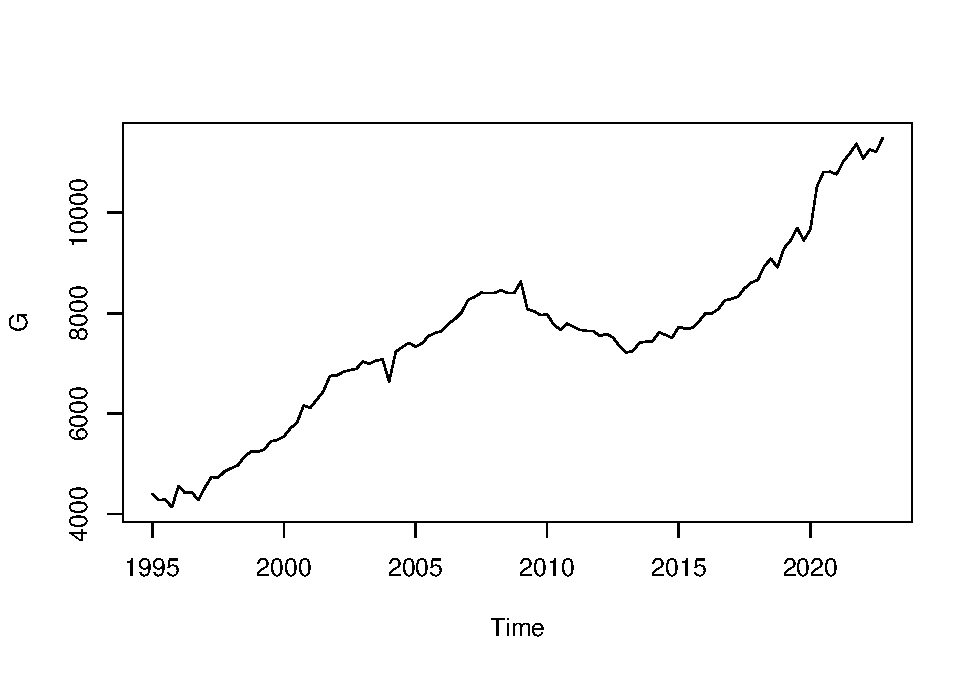
\includegraphics{AdvMacro2_Assignment1_files/figure-latex/unnamed-chunk-2-4.pdf}
\#\# Sample Statistics Let's compute the sample means:

\begin{Shaded}
\begin{Highlighting}[]
\NormalTok{CdivGDP }\OtherTok{\textless{}{-}}\NormalTok{ C}\SpecialCharTok{/}\NormalTok{GDP}
\NormalTok{IdivGDP }\OtherTok{\textless{}{-}}\NormalTok{ I}\SpecialCharTok{/}\NormalTok{GDP}
\NormalTok{GdivGDP }\OtherTok{\textless{}{-}}\NormalTok{ G}\SpecialCharTok{/}\NormalTok{GDP}

\FunctionTok{mean}\NormalTok{(CdivGDP)}
\end{Highlighting}
\end{Shaded}

\begin{verbatim}
## [1] 0.4063485
\end{verbatim}

\begin{Shaded}
\begin{Highlighting}[]
\FunctionTok{mean}\NormalTok{(IdivGDP)}
\end{Highlighting}
\end{Shaded}

\begin{verbatim}
## [1] 0.2530171
\end{verbatim}

\begin{Shaded}
\begin{Highlighting}[]
\FunctionTok{mean}\NormalTok{(GdivGDP)}
\end{Highlighting}
\end{Shaded}

\begin{verbatim}
## [1] 0.1719054
\end{verbatim}

\hypertarget{detrending}{%
\subsection{Detrending}\label{detrending}}

Let's apply the HP filter:

\begin{Shaded}
\begin{Highlighting}[]
\FunctionTok{plot}\NormalTok{(}\FunctionTok{hpfilter}\NormalTok{(}\FunctionTok{log}\NormalTok{(GDP)))}
\end{Highlighting}
\end{Shaded}

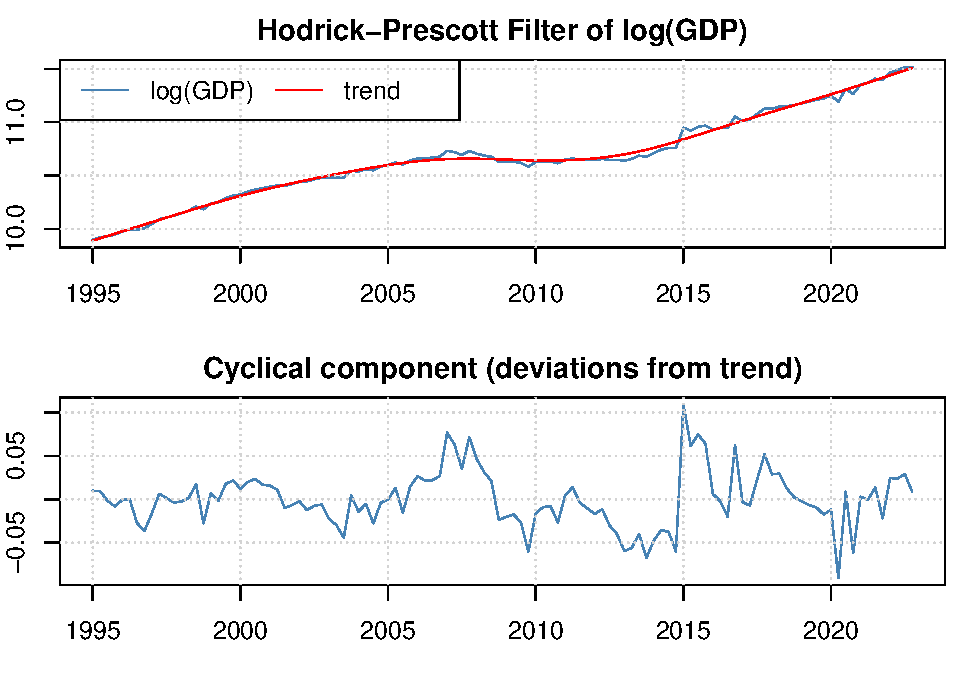
\includegraphics{AdvMacro2_Assignment1_files/figure-latex/unnamed-chunk-4-1.pdf}

\begin{Shaded}
\begin{Highlighting}[]
\FunctionTok{plot}\NormalTok{(}\FunctionTok{hpfilter}\NormalTok{(}\FunctionTok{log}\NormalTok{(G)))}
\end{Highlighting}
\end{Shaded}

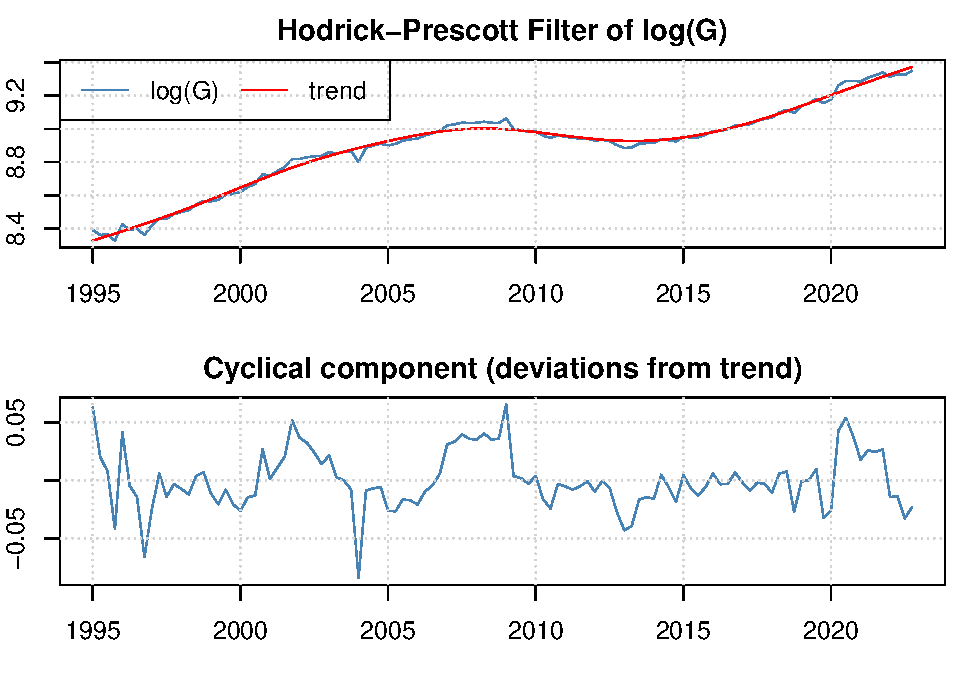
\includegraphics{AdvMacro2_Assignment1_files/figure-latex/unnamed-chunk-4-2.pdf}

\begin{Shaded}
\begin{Highlighting}[]
\FunctionTok{plot}\NormalTok{(}\FunctionTok{hpfilter}\NormalTok{(}\FunctionTok{log}\NormalTok{(I)))}
\end{Highlighting}
\end{Shaded}

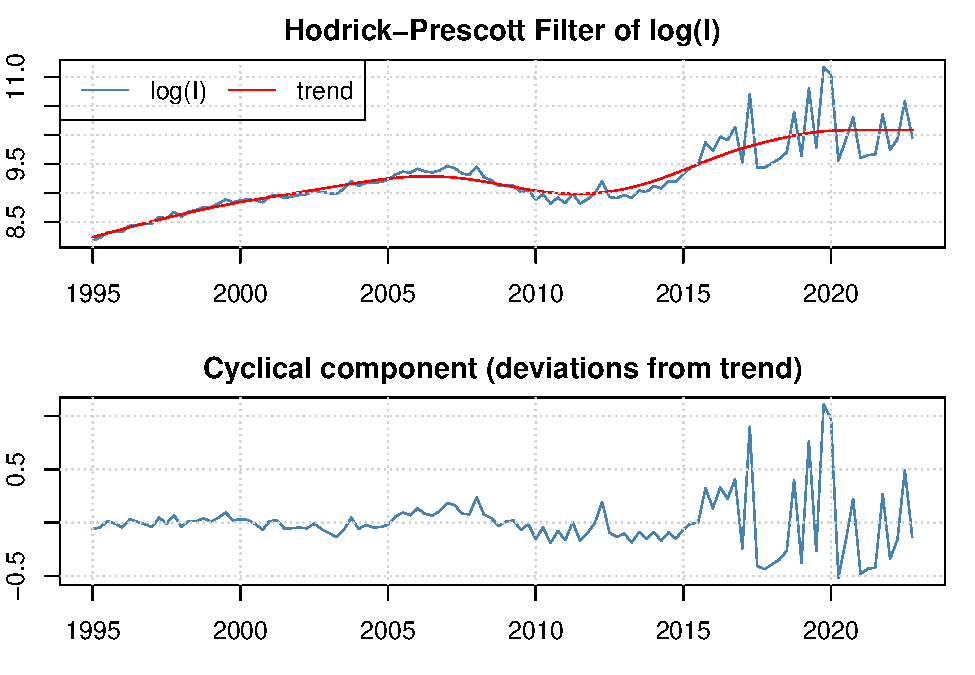
\includegraphics{AdvMacro2_Assignment1_files/figure-latex/unnamed-chunk-4-3.pdf}

\begin{Shaded}
\begin{Highlighting}[]
\FunctionTok{plot}\NormalTok{(}\FunctionTok{hpfilter}\NormalTok{(}\FunctionTok{log}\NormalTok{(C)))}
\end{Highlighting}
\end{Shaded}

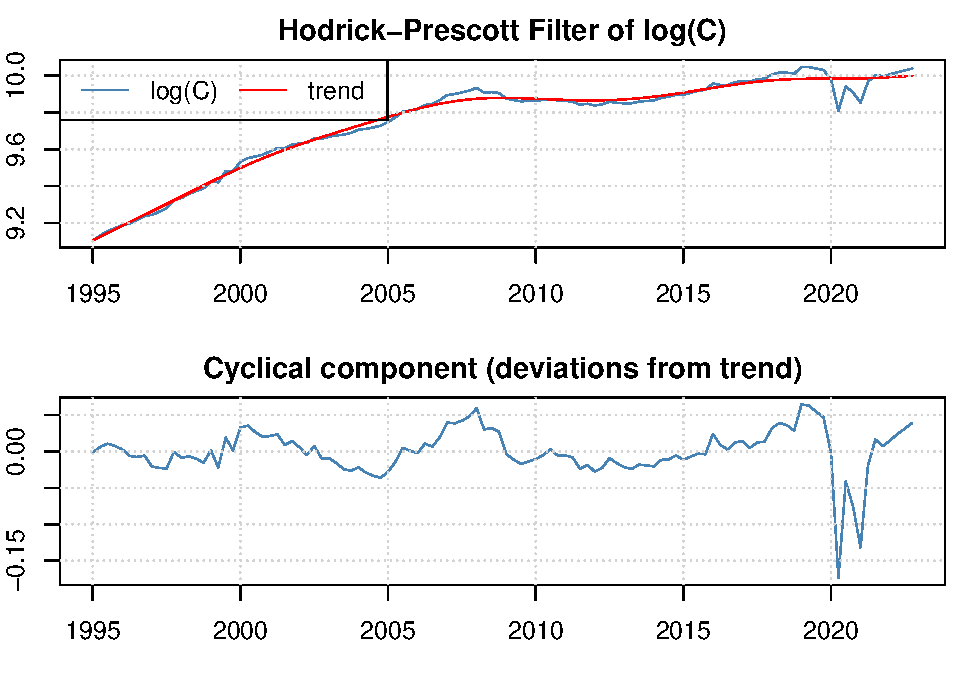
\includegraphics{AdvMacro2_Assignment1_files/figure-latex/unnamed-chunk-4-4.pdf}

\hypertarget{business-cycle-stylized-facts}{%
\subsection{Business Cycle Stylized
Facts}\label{business-cycle-stylized-facts}}

\begin{Shaded}
\begin{Highlighting}[]
\NormalTok{trend\_G }\OtherTok{\textless{}{-}} \FunctionTok{hpfilter}\NormalTok{(}\FunctionTok{log}\NormalTok{(G))[}\DecValTok{1}\NormalTok{]}\SpecialCharTok{$}\NormalTok{cycle}
\NormalTok{trend\_C }\OtherTok{\textless{}{-}} \FunctionTok{hpfilter}\NormalTok{(}\FunctionTok{log}\NormalTok{(C))[}\DecValTok{1}\NormalTok{]}\SpecialCharTok{$}\NormalTok{cycle}
\NormalTok{trend\_I }\OtherTok{\textless{}{-}} \FunctionTok{hpfilter}\NormalTok{(}\FunctionTok{log}\NormalTok{(I))[}\DecValTok{1}\NormalTok{]}\SpecialCharTok{$}\NormalTok{cycle}
\NormalTok{trend\_GDP }\OtherTok{\textless{}{-}} \FunctionTok{hpfilter}\NormalTok{(}\FunctionTok{log}\NormalTok{(GDP))[}\DecValTok{1}\NormalTok{]}\SpecialCharTok{$}\NormalTok{cycle}

\NormalTok{output\_table }\OtherTok{\textless{}{-}} \FunctionTok{data.frame}\NormalTok{(}
  \AttributeTok{names =} \FunctionTok{c}\NormalTok{(}\StringTok{"GDP"}\NormalTok{,}\StringTok{"I"}\NormalTok{,}\StringTok{"C"}\NormalTok{,}\StringTok{"G"}\NormalTok{),}
  \AttributeTok{standard\_deviation =} \FunctionTok{c}\NormalTok{(}\FunctionTok{sd}\NormalTok{(trend\_GDP),}\FunctionTok{sd}\NormalTok{(trend\_I),}\FunctionTok{sd}\NormalTok{(trend\_C),}\FunctionTok{sd}\NormalTok{(trend\_G)),}
  \AttributeTok{relative\_sd =} \FunctionTok{c}\NormalTok{(}\FunctionTok{sd}\NormalTok{(trend\_GDP)}\SpecialCharTok{/}\FunctionTok{sd}\NormalTok{(trend\_GDP),}\FunctionTok{sd}\NormalTok{(trend\_I)}\SpecialCharTok{/}\FunctionTok{sd}\NormalTok{(trend\_GDP), }\FunctionTok{sd}\NormalTok{(trend\_C)}\SpecialCharTok{/}\FunctionTok{sd}\NormalTok{(trend\_GDP),}\FunctionTok{sd}\NormalTok{(trend\_G)}\SpecialCharTok{/}\FunctionTok{sd}\NormalTok{(trend\_GDP)),}
  \AttributeTok{cont\_output\_corr =} \FunctionTok{c}\NormalTok{(}\FunctionTok{cor}\NormalTok{(trend\_GDP,trend\_GDP), }\FunctionTok{cor}\NormalTok{(trend\_I,trend\_GDP), }\FunctionTok{cor}\NormalTok{(trend\_C,trend\_GDP), }\FunctionTok{cor}\NormalTok{(trend\_G,trend\_GDP))}
\NormalTok{    )}
\NormalTok{output\_table}
\end{Highlighting}
\end{Shaded}

\begin{verbatim}
##   names standard_deviation relative_sd cont_output_corr
## 1   GDP         0.03230920   1.0000000        1.0000000
## 2     I         0.25468238   7.8826591        0.1112197
## 3     C         0.03193810   0.9885142        0.4768935
## 4     G         0.02470573   0.7646655        0.1549818
\end{verbatim}

\hypertarget{window-1}{%
\subsubsection{Window 1}\label{window-1}}

\begin{Shaded}
\begin{Highlighting}[]
\NormalTok{GDP\_W1 }\OtherTok{\textless{}{-}} \FunctionTok{window}\NormalTok{(GDP, }\AttributeTok{end=}\FloatTok{2007.75}\NormalTok{)}
\NormalTok{I\_W1 }\OtherTok{\textless{}{-}} \FunctionTok{window}\NormalTok{(I, }\AttributeTok{end=}\FloatTok{2007.75}\NormalTok{)}
\NormalTok{C\_W1 }\OtherTok{\textless{}{-}} \FunctionTok{window}\NormalTok{(C, }\AttributeTok{end=}\FloatTok{2007.75}\NormalTok{)}
\NormalTok{G\_W1 }\OtherTok{\textless{}{-}} \FunctionTok{window}\NormalTok{(G, }\AttributeTok{end=}\FloatTok{2007.75}\NormalTok{)}

\NormalTok{trend\_G }\OtherTok{\textless{}{-}} \FunctionTok{hpfilter}\NormalTok{(}\FunctionTok{log}\NormalTok{(G\_W1))[}\DecValTok{1}\NormalTok{]}\SpecialCharTok{$}\NormalTok{cycle}
\NormalTok{trend\_C }\OtherTok{\textless{}{-}} \FunctionTok{hpfilter}\NormalTok{(}\FunctionTok{log}\NormalTok{(C\_W1))[}\DecValTok{1}\NormalTok{]}\SpecialCharTok{$}\NormalTok{cycle}
\NormalTok{trend\_I }\OtherTok{\textless{}{-}} \FunctionTok{hpfilter}\NormalTok{(}\FunctionTok{log}\NormalTok{(I\_W1))[}\DecValTok{1}\NormalTok{]}\SpecialCharTok{$}\NormalTok{cycle}
\NormalTok{trend\_GDP }\OtherTok{\textless{}{-}} \FunctionTok{hpfilter}\NormalTok{(}\FunctionTok{log}\NormalTok{(GDP\_W1))[}\DecValTok{1}\NormalTok{]}\SpecialCharTok{$}\NormalTok{cycle}

\NormalTok{output\_table\_W1 }\OtherTok{\textless{}{-}} \FunctionTok{data.frame}\NormalTok{(}
  \AttributeTok{names =} \FunctionTok{c}\NormalTok{(}\StringTok{"GDP"}\NormalTok{,}\StringTok{"I"}\NormalTok{,}\StringTok{"C"}\NormalTok{,}\StringTok{"G"}\NormalTok{),}
  \AttributeTok{standard\_deviation =} \FunctionTok{c}\NormalTok{(}\FunctionTok{sd}\NormalTok{(trend\_GDP),}\FunctionTok{sd}\NormalTok{(trend\_I),}\FunctionTok{sd}\NormalTok{(trend\_C),}\FunctionTok{sd}\NormalTok{(trend\_G)),}
  \AttributeTok{relative\_sd =} \FunctionTok{c}\NormalTok{(}\FunctionTok{sd}\NormalTok{(trend\_GDP)}\SpecialCharTok{/}\FunctionTok{sd}\NormalTok{(trend\_GDP),}\FunctionTok{sd}\NormalTok{(trend\_I)}\SpecialCharTok{/}\FunctionTok{sd}\NormalTok{(trend\_GDP), }\FunctionTok{sd}\NormalTok{(trend\_C)}\SpecialCharTok{/}\FunctionTok{sd}\NormalTok{(trend\_GDP),}\FunctionTok{sd}\NormalTok{(trend\_G)}\SpecialCharTok{/}\FunctionTok{sd}\NormalTok{(trend\_GDP)),}
  \AttributeTok{cont\_output\_corr =} \FunctionTok{c}\NormalTok{(}\FunctionTok{cor}\NormalTok{(trend\_GDP,trend\_GDP), }\FunctionTok{cor}\NormalTok{(trend\_I,trend\_GDP), }\FunctionTok{cor}\NormalTok{(trend\_C,trend\_GDP), }\FunctionTok{cor}\NormalTok{(trend\_G,trend\_GDP))}
\NormalTok{  )}
\end{Highlighting}
\end{Shaded}

\hypertarget{window-2}{%
\subsubsection{Window 2}\label{window-2}}

\begin{Shaded}
\begin{Highlighting}[]
\NormalTok{GDP\_W2 }\OtherTok{\textless{}{-}} \FunctionTok{window}\NormalTok{(GDP, }\AttributeTok{start=}\FloatTok{2008.0}\NormalTok{)}
\NormalTok{I\_W2 }\OtherTok{\textless{}{-}} \FunctionTok{window}\NormalTok{(I, }\AttributeTok{start=}\FloatTok{2008.0}\NormalTok{)}
\NormalTok{C\_W2 }\OtherTok{\textless{}{-}} \FunctionTok{window}\NormalTok{(C, }\AttributeTok{start=}\FloatTok{2008.0}\NormalTok{)}
\NormalTok{G\_W2 }\OtherTok{\textless{}{-}} \FunctionTok{window}\NormalTok{(G, }\AttributeTok{start=}\FloatTok{2008.0}\NormalTok{)}

\NormalTok{trend\_G }\OtherTok{\textless{}{-}} \FunctionTok{hpfilter}\NormalTok{(}\FunctionTok{log}\NormalTok{(G\_W2))[}\DecValTok{1}\NormalTok{]}\SpecialCharTok{$}\NormalTok{cycle}
\NormalTok{trend\_C }\OtherTok{\textless{}{-}} \FunctionTok{hpfilter}\NormalTok{(}\FunctionTok{log}\NormalTok{(C\_W2))[}\DecValTok{1}\NormalTok{]}\SpecialCharTok{$}\NormalTok{cycle}
\NormalTok{trend\_I }\OtherTok{\textless{}{-}} \FunctionTok{hpfilter}\NormalTok{(}\FunctionTok{log}\NormalTok{(I\_W2))[}\DecValTok{1}\NormalTok{]}\SpecialCharTok{$}\NormalTok{cycle}
\NormalTok{trend\_GDP }\OtherTok{\textless{}{-}} \FunctionTok{hpfilter}\NormalTok{(}\FunctionTok{log}\NormalTok{(GDP\_W2))[}\DecValTok{1}\NormalTok{]}\SpecialCharTok{$}\NormalTok{cycle}

\NormalTok{output\_table\_W2 }\OtherTok{\textless{}{-}} \FunctionTok{data.frame}\NormalTok{(}
  \AttributeTok{names =} \FunctionTok{c}\NormalTok{(}\StringTok{"GDP"}\NormalTok{,}\StringTok{"I"}\NormalTok{,}\StringTok{"C"}\NormalTok{,}\StringTok{"G"}\NormalTok{),}
  \AttributeTok{standard\_deviation =} \FunctionTok{c}\NormalTok{(}\FunctionTok{sd}\NormalTok{(trend\_GDP),}\FunctionTok{sd}\NormalTok{(trend\_I),}\FunctionTok{sd}\NormalTok{(trend\_C),}\FunctionTok{sd}\NormalTok{(trend\_G)),}
  \AttributeTok{relative\_sd =} \FunctionTok{c}\NormalTok{(}\FunctionTok{sd}\NormalTok{(trend\_GDP)}\SpecialCharTok{/}\FunctionTok{sd}\NormalTok{(trend\_GDP),}\FunctionTok{sd}\NormalTok{(trend\_I)}\SpecialCharTok{/}\FunctionTok{sd}\NormalTok{(trend\_GDP), }\FunctionTok{sd}\NormalTok{(trend\_C)}\SpecialCharTok{/}\FunctionTok{sd}\NormalTok{(trend\_GDP),}\FunctionTok{sd}\NormalTok{(trend\_G)}\SpecialCharTok{/}\FunctionTok{sd}\NormalTok{(trend\_GDP)),}
  \AttributeTok{cont\_output\_corr =} \FunctionTok{c}\NormalTok{(}\FunctionTok{cor}\NormalTok{(trend\_GDP,trend\_GDP), }\FunctionTok{cor}\NormalTok{(trend\_I,trend\_GDP), }\FunctionTok{cor}\NormalTok{(trend\_C,trend\_GDP), }\FunctionTok{cor}\NormalTok{(trend\_G,trend\_GDP))}
\NormalTok{    )}
\end{Highlighting}
\end{Shaded}

\hypertarget{output}{%
\subsubsection{Output}\label{output}}

\begin{Shaded}
\begin{Highlighting}[]
\NormalTok{output\_table}
\end{Highlighting}
\end{Shaded}

\begin{verbatim}
##   names standard_deviation relative_sd cont_output_corr
## 1   GDP         0.03230920   1.0000000        1.0000000
## 2     I         0.25468238   7.8826591        0.1112197
## 3     C         0.03193810   0.9885142        0.4768935
## 4     G         0.02470573   0.7646655        0.1549818
\end{verbatim}

\begin{Shaded}
\begin{Highlighting}[]
\NormalTok{output\_table\_W1}
\end{Highlighting}
\end{Shaded}

\begin{verbatim}
##   names standard_deviation relative_sd cont_output_corr
## 1   GDP         0.01582877    1.000000        1.0000000
## 2     I         0.05050510    3.190716        0.4005525
## 3     C         0.01591679    1.005561        0.4630622
## 4     G         0.02558119    1.616120        0.1368501
\end{verbatim}

\begin{Shaded}
\begin{Highlighting}[]
\NormalTok{output\_table\_W2}
\end{Highlighting}
\end{Shaded}

\begin{verbatim}
##   names standard_deviation relative_sd cont_output_corr
## 1   GDP         0.03803500   1.0000000      1.000000000
## 2     I         0.34357331   9.0330832      0.054996823
## 3     C         0.03783447   0.9947279      0.392198387
## 4     G         0.01911173   0.5024774      0.006569063
\end{verbatim}

\hypertarget{question-2-a-real-business-cycle-model-with-energy-price-shocks-5-points}{%
\section{Question 2: A real business cycle model with energy price
shocks (5
points)}\label{question-2-a-real-business-cycle-model-with-energy-price-shocks-5-points}}

Expected discounted utility of the representative household:
\begin{equation}
  U = E_0\left[\sum_{t=0}^\infty\beta_t\frac{C_t^{1-\sigma}}{1-\sigma}+\theta \log(1-N_t)\right]
\end{equation} subject to \begin{equation}
  C_t + K_{t+1}+P_tEN_t \leq A_tK_t^\alpha N_t^\gamma EN_t^{1-\alpha-\gamma}+(1-\delta)K_t
\end{equation}

\hypertarget{a}{%
\subsection{(a)}\label{a}}

\hypertarget{question-3-understanding-impulse-responses-and-model-simulation-total-of-8-points}{%
\section{Question 3: Understanding impulse responses and model
simulation (total of 8
points)}\label{question-3-understanding-impulse-responses-and-model-simulation-total-of-8-points}}

Set up the Lagrange System: \[L = E_t \left[ 
\begin{array} \alpha = a\\ b=
\end{array} 
\right]\]

\end{document}
